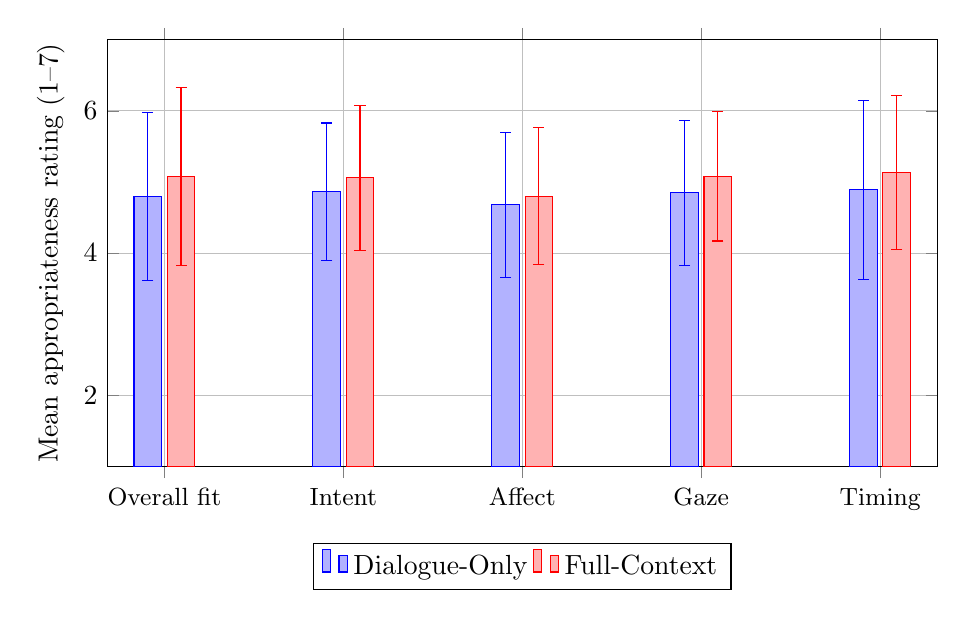
\begin{tikzpicture}
\begin{axis}[
    ybar,
    width=\textwidth,
    height=7.0cm,
    ymin=1, ymax=7,
    ylabel={Mean appropriateness rating (1--7)},
    symbolic x coords={Overall fit,Intent,Affect,Gaze,Timing},
    xtick=data,
    x tick label style={font=\small},
    legend style={at={(0.5,-0.18)},anchor=north,legend columns=2},
    error bars/y dir=both,error bars/y explicit,
    bar width=10pt,
    enlarge x limits=0.08,
    grid=major,
]
\addplot+ coordinates {
(Overall fit,4.80) +- (0,1.18)
(Intent,4.86) +- (0,0.97)
(Affect,4.68) +- (0,1.02)
(Gaze,4.85) +- (0,1.02)
(Timing,4.89) +- (0,1.26)
};
\addplot+ coordinates {
(Overall fit,5.08) +- (0,1.25)
(Intent,5.06) +- (0,1.02)
(Affect,4.80) +- (0,0.96)
(Gaze,5.08) +- (0,0.91)
(Timing,5.13) +- (0,1.08)
};
\legend{Dialogue-Only,Full-Context}
\end{axis}
\end{tikzpicture}
